\subsection{Detector Support System}
\label{sec:fdsp-tc-infr-dss}

The \dword{dss} provides the structural support for the \dword{spmod} inside the cryostat.  
It also provides the necessary infrastructure to move the detector elements into place during
assembly. 
The \dword{dss} is a new design, quite different from the \dword{pdsp} \dword{dss}. It is described in some detail in this
section. 
The detector elements supported by the \dword{dss} include the \dwords{ewfc}, the \dwords{apa}, and the \dwords{cpa} with top and bottom \dword{fc} panels. The nominal load of the detector elements both dry (in air) and wet (under \dword{lar}) are shown in Table \ref{tab:installation-DSS-load}. The weights listed are the current design weights and do not include any margin for future design changes.  
The \dword{dss}, however, is designed so the weights can be doubled, and it would still meet the requirements of the design codes.  
Deformations would increase due to any increase in loads, and this effect should be evaluated.
\begin{dunetable}
[DSS Loads]
{l|c|cc|cc}
{tab:installation-DSS-load}
{The expected dry and wet stratic loads for the DSS.}
%\multicolumn{2}{c}{} &  \multicolumn{4}{|c}{Dry Weight}\\ \toprowrule
& &  \multicolumn{4}{|c}{Dry Weight}\\ \toprowrule
& & \multicolumn{2}{c|}{Unit Weight} & \multicolumn{2}{c|}{Total Weight}  \\ \colhline

Detector Component &\# Units& (kg)&(lbs) & (kg) &(lbs)\\ \colhline
Detector Support Structure (DSS) (not in liquid) & 1 &NA&NA& 12318  & 27100 \\ 
\colhline
Anode Plane Assembly (Installed APA pair/No cables)& 75&1184 &2604 &88768  &195290\\ 
\colhline
Cathode Plane Assembly (CPA) & 100& 233 & 513 & 23331 & 51327 \\ 
\colhline
Top or Bottom Field Cage module (FC TB)& 400&149 & 328	 & 59679 & 131294\\ 
\colhline
CE Cables &750& 182 & 400 & 13636 & 30000\\
\colhline
Field Cage Endwall  & 8	&904 &	1989  & 7234 & 15914\\ 
\colhline
{\bf Total} &  & & & 204966 &	450925\\ 
\colhline
\toprowrule

 & &  \multicolumn{4}{c}{Wet Weight}\\
\toprowrule
Detector Support Structure (DSS) (not in liquid) & 1 & NA & NA & 12318 & 27100 \\ 
\colhline
Anode Plane Assembly (Installed APA pair/No cables)&75& &0 & 0 &0\\ 
\colhline
Cathode Plane Assembly (CPA) & 100& 45 & 99 & 4520 & 9943 \\ 
\colhline
Top or Bottom Field Cage module (FC TB)& 400 & 68 & 150	& 27359 & 60191 \\ 
\colhline
CE Cables & 75 & & & 13636& 30000 \\
\colhline
Field Cage Endwall & 8 & 283& 	622& 2263 & 4978\\  
\colhline
{\bf Total} &  & & &60096	 &132211 \\ 
\colhline
\end{dunetable}


\begin{dunefigure}[\threed model of the \dword{dss} ]{fig:DSS}
  {\threed model of the \dword{dss} showing the entire
  structure on the left along with one \dword{apa} row and one
  \dword{cpa}-\dword{fc} row at each end. The right panel is a zoomed image
  showing the connections between the vertical supports and the
  horizontal I-beams.}
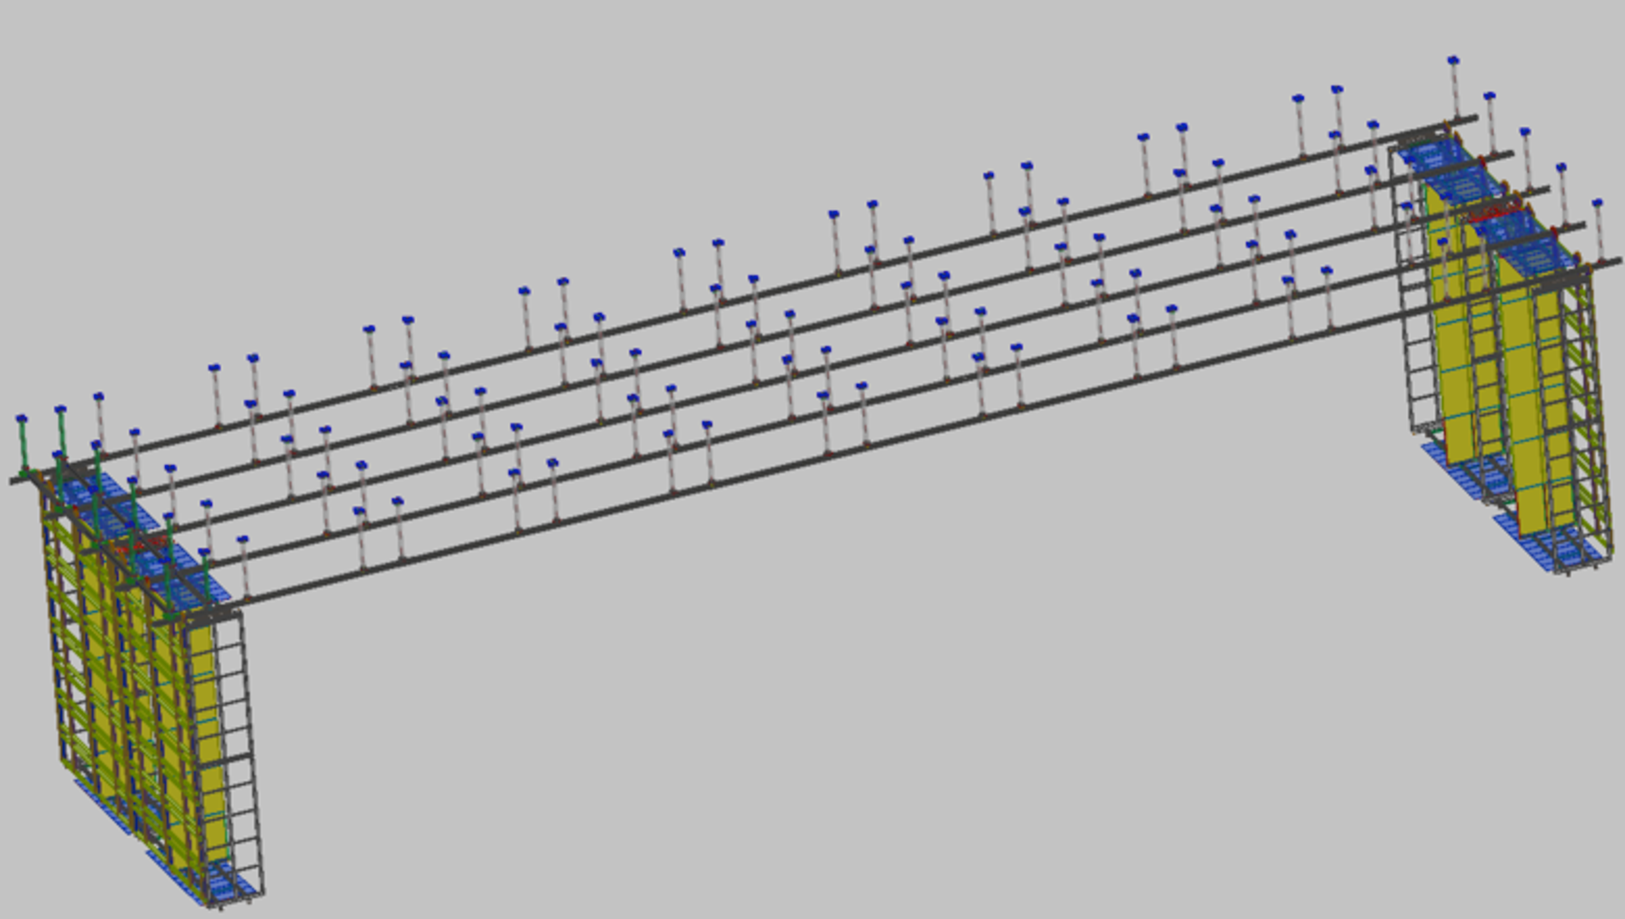
\includegraphics[width=.49\textwidth]{DSS-1.pdf}
 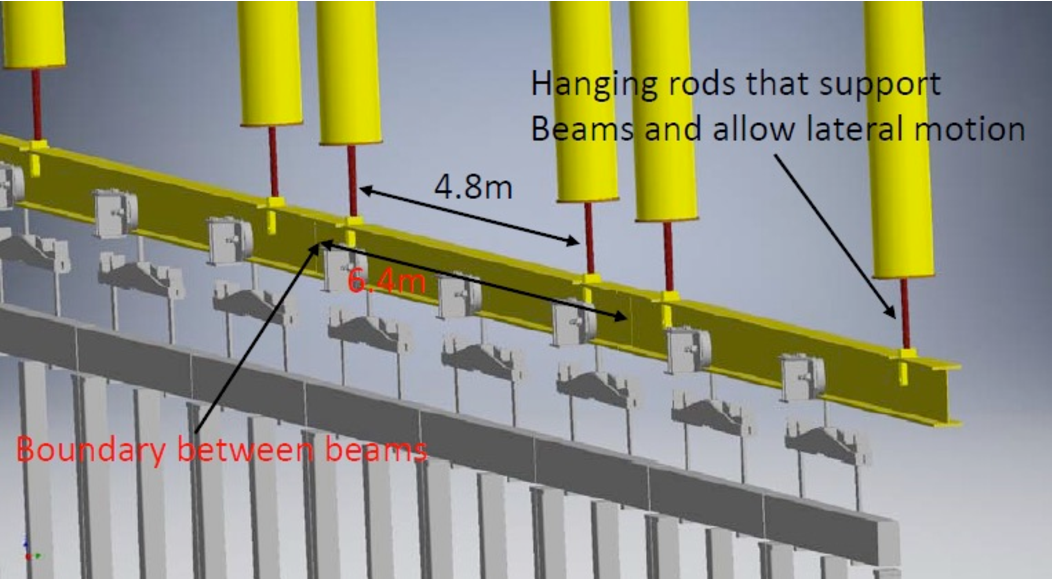
\includegraphics[width=.49\textwidth]{DSS-2.pdf}
\end{dunefigure}

The \dword{dss} is supported by the
cryostat outer steel structure through a series of \fdth{}s that cross through the cryostat insulation and anchored with flanges on
the cryostat roof. 
Inside the cryostat, a series of stainless steel I-beams are connected to the \fdth{}s and used to support the
detector. 
The \dword{dss} defines the location of the detector inside the cryostat and also defines how the detector elements move and contract as the detector is brought to \dword{lar} temperature. 
The design of the \dword{dss} encompasses the overall
structural design of the \dword{detmodule} because only after the elements are mounted to the \dword{dss} and connected do they make a unified mechanical structure. 
Figure~\ref{fig:DSS} (left) shows the \dword{dss} structure; there are
five rows of supports for the alternating rows of
\dword{apa}-\dword{cpa}-\dword{apa}-\dword{cpa}-\dword{apa}.  
The \dword{dss} is connected to the cryostat warm structure at a flange mounted on the outside of the cryostat.  
Figure~\ref{fig:DSS} (right)
shows the layout of these structural \fdth{}s.

The \dword{dss} is designed to meet the following  requirements:
\begin{itemize}
 \setlength\itemsep{1mm}
\setlength{\parsep}{1mm}
\setlength{\itemsep}{-5mm}
% \small
\item Support the weight of the detector;
\item Accommodate cryostat roof movement during filling, testing, and operation;
\item Accommodate variation in \fdth locations and
  variation in the flange angles due to installation tolerances and
  loading on the warm structure;
\item Accommodate shrinkage of the detector and \dword{dss} from ambient
  temperature to \dword{lar} temperature;
\item Define the positions of the detector components relative to each other; 
\item Provide electrical connection to the cryostat ground and remain electrically isolated from the detector;
\item Allow support penetrations to be purged with gaseous argon to prevent contaminants from diffusing back into the liquid; 
\item Ensure that the instrumentation cabling does not interfere with the \dword{dss};
\item Consist entirely of components that can  
be installed through the \dword{tco};
\item %Design to m
Meet AISC-360 or appropriate codes required at \dword{surf};
\item %Design to m
Meet seismic requirements one mile underground at \dword{surf};
\item Consist entirely of %All materials must be 
materials compatible for operation in ultrapure \dword{lar};
\item Ensure that beams are completely submerged in \dword{lar};
\item Ensure that detector components are not less than \SI{400}{mm} from the membrane flat surface;
\item Ensure that the supports do not interfere with the cryostat I-beam structures;
\item Ensure %Design such 
that the detector's lower \dword{gp} is lies over the cryogenic piping and that the tops of the \dword{dss} beams are submerged in \dword{lar} while leaving a \SI{4}{\%} ullage at the top of the cryostat;
\item Include the infrastructure necessary to move the \dword{apa} and
  \dword{cpa}-\dword{fc} assemblies from outside the cryostat through the
  \dword{tco} and to the correct position.
\end{itemize}

  The \dword{dss}
consists of pairs of \fdth{}s that support \SI{6.4}{m}-long
W10x26 stainless steel I-beam sections. The proposed design of the
\dword{dss} has \num{10} I-beam segments per row for a total of
\num{50} I-beam segments. Each I-beam is suspended on both ends by
rods from \fdth{}s that penetrate the cryostat roof.  %In the cold condition
When cold, each I-beam shrinks, causing gaps to form between
\dword{apa}s that are adjacent but supported on separate beams.
\dword{apa}s that are supported on the same beam will not have gaps
develop because both the beam and \dword{apa}s are stainless steel so
they shrink together.  Each beam is supported by a nearly
\SI{2}{m} long rod that allows the beam support to move as the beam
contracts.


The feedthrough consists of a flange and $6 ^{''}$ OD structural tube welded to it that extends through the cryostat insulation.  
There is a
nominal \SI{10}{mm} gap between the OD of the tube and the ID of the clearance tube in the cryostat. \fixme{OD and ID are not defined in the common glossary.}
The $6 ^{''}$ tube provides lateral support to the I-beams during installation.
Running down the center of the feedthrough is a $1^{"}$ diameter rod supported at a swivel washer at the flange and then supported by the
I-beam at a clevis.  The gas seal is obtained by Conflat Flange and a
bellows that seals around the swivel washer.  The lateral position and height of the rod can be adjusted $\pm$1 inch to accommodate tolerances in positioning cryostat crossing tubes. Figure \ref{fig:DSS-lateral-support} shows the end of the $6 ^{''}$ tube and how it locks the I-Beam into position. 

\begin{dunefigure}[DSS support for lateral loads ]{fig:DSS-lateral-support}
  {Left panel shows how the central support rod is locked in postion during detector installation. The outer $6 ^{''}$ tube is used to fix the support clevis in position. The right panel shows the system as it is connected to the I-Beam.}
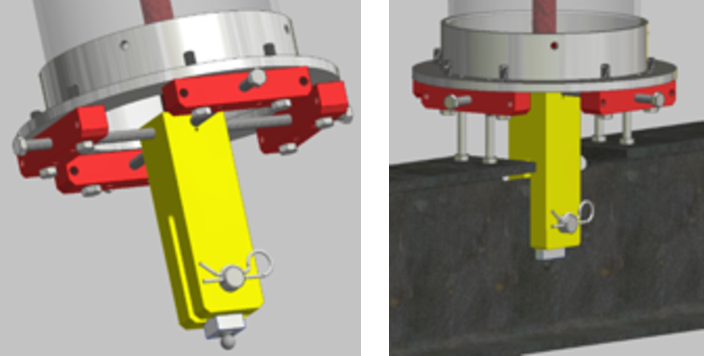
\includegraphics[width=.75\textwidth]{graphics/dss-lateral-support.pdf}
\end{dunefigure}

After the detector has been installed all restraints will be released to allow motion as the detector contracts during cool down.  The two hangars that support each \dword{dss} beam will contract and move toward each other by 13.1 mm along the axis of the detector.  
The drift distance will shrink by 7.4mm caused by the contraction of the field cages.  The detector is symmetric in the drift direction around the center \dword{apa}.  The drifts on either side of the center \dword{apa} will  shrink toward the center while the center \dword{apa} remains unmoved.  This results in the \dwords{cpa} moving 7.4mm toward the center and the outer \dword{apa}s moving 14.8mm (2*7.4mm) toward the center.  The hanging rod is designed to have a range of motion of 15mm in the drift direction to accommodate this shrinkage.




Detector components are installed using a shuttle beam system as
illustrated in Figure~\ref{fig:shuttle}.  
The last two columns of
\fdth{}s (eastern-most) support temporary beams that run
north-south, perpendicular to the main \dword{dss} beams.  
A shuttle beam has trolleys mounted to it and transverses 
north-south until it aligns with the required row of \dword{dss} beams.  
The last \dword{apa} or \dword{cpa} in a row is supported by the shuttle beam, which is bolted directly to the \fdth{}s once it is in place.  
As the last \dword{cpa} or \dword{apa} in each row is installed, the north-south beams are removed.

\begin{dunefigure}[\threed models of the shuttle beam end of the \dword{dss}]{fig:shuttle}
  {\threed models of the shuttle beam end of the \dword{dss}. The figures show how an \dword{apa}
is translated into position using the north-south beams until it lines up with the correct
row of I-beams.}
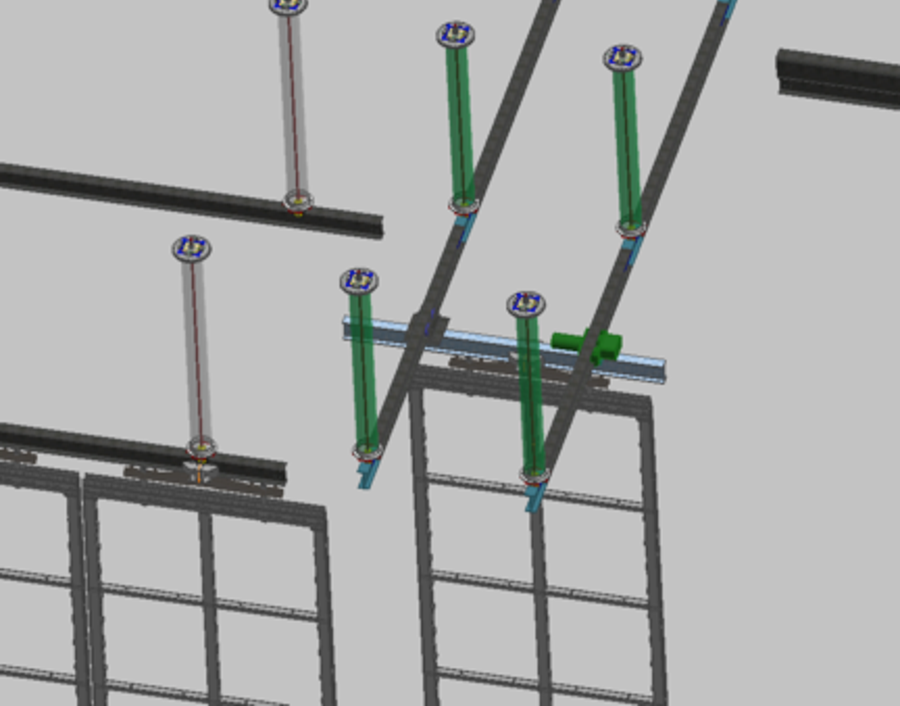
\includegraphics[width=.49\textwidth]{/Shuttle-1.pdf}
 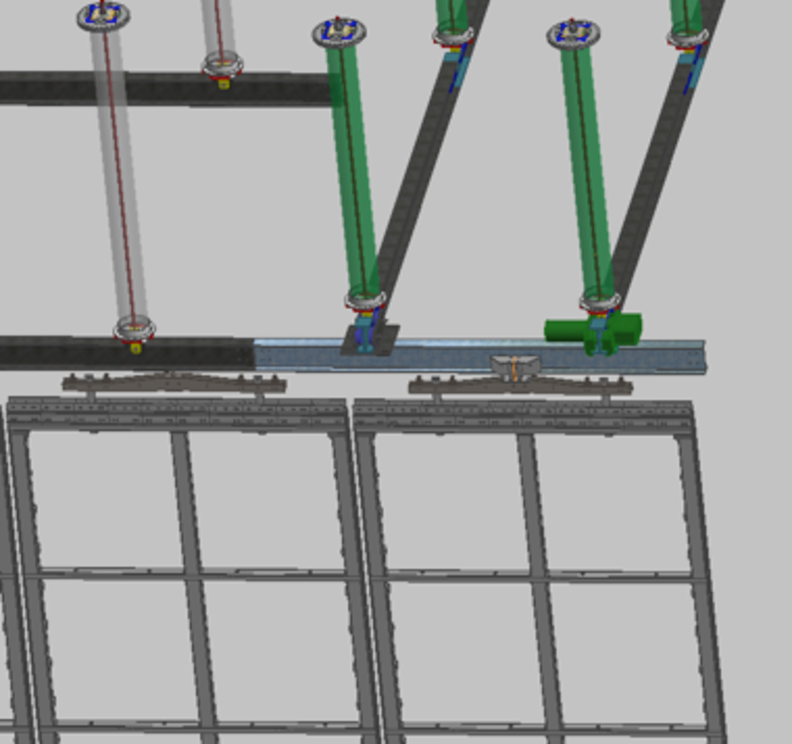
\includegraphics[width=.42\textwidth]{shuttle-2.pdf}
\end{dunefigure}

A mechanical interlock system  prevents trolleys
from passing the end of the shuttle beam unless it is aligned with a
corresponding \dword{dss} beam.  The shuttle beam and each detector component are
moved using a motorized trolley.  A commercially available motorized
trolley will be modified as needed for the
installation. 




\begin{dunefigure}[Prototype of the motorized DSS trolley ]{fig:DSS-trolley}
  {Prototype of the motorized DSS trolley that will push the APA and CPA along the I-beams and through the switchyard.}
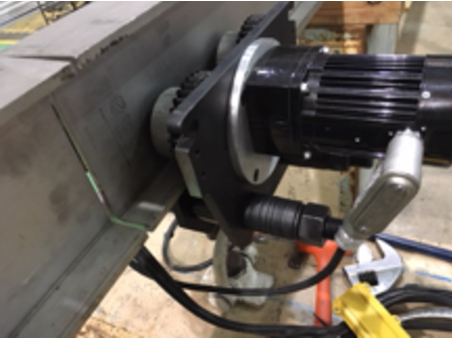
\includegraphics[width=.49\textwidth]{graphics/DSS-trolley.pdf}
\end{dunefigure}



A mock-up of the shuttle system will be constructed to test the
mechanical interlock and drive systems for the shuttle beam
for each \dword{detmodule}.  Tests will be conducted to evaluate the level of
misalignment between beams that can be tolerated and the amount of
positional control that can be achieved with the motorized trolley. We plan to construct a full scale prototype of a section of the  switchyard and perform tests at floor level. Later, the test program will be expanded at Ash River, where a full scale installation test will be performed. This is described in the installation \dword{qa} section.
